\documentclass[11pt]{article}

\usepackage{ulem}
\usepackage{tikz}
\usepackage{xurl}
\usepackage{float}
\usepackage{amsmath}
\usepackage{booktabs}
\usepackage{graphicx}
\usepackage{listings}
\usepackage[T5]{fontenc}
\usepackage{indentfirst}
\usepackage[utf8]{inputenc}
\usepackage[margin=1in]{geometry}
\usetikzlibrary{arrows.meta, positioning}

\begin{document}

\begin{center}

{\Large \textbf{UNIVERSITY OF SCIENCE AND TECHNOLOGY OF HANOI}}\\
\vspace{0.3cm}
----------------------o0o----------------------\\

\vspace{4cm}

{\large
\centerline{2540027 - Nguyễn Xuân Vinh}
}

\vspace{4cm}

{\Huge \textbf{BC3.04a Advanced Programming for HPC}}\\
\vspace{0.5cm}
Lecturer: Dr. Trần Giang Sơn

\vspace{4cm}

{\Large \textbf{REPORT LABWORK 7}}\\

\vspace{0.5cm}

{\large
Subjects: Reduction
}

\vspace{4cm}
\today
\end{center}

\newpage

\newpage

\tableofcontents

\newpage

\section{Objective}

The objective of the labwork 7 is to implement grayscale stretching using a Map-Reduce style approach. The grayscale stretch consists of three main steps:

\begin{enumerate}
\item Convert the input image to grayscale using a Map operation.
\item Find the minimum and maximum grayscale intensities using a Reduce operation.
\item Linearly recalculate the intensity of each pixel using another Map operation.
\end{enumerate}

Different 2D block sizes are also tested to measure their execution time.

\section{Implementation}

The input image was loaded from \texttt{/content/img.jpg} using OpenCV. The image has a size of $1080 \times 1920$ pixels with three color channels.

The implementation uses a block-based processing function. The image is divided into 2D blocks, and the corresponding operation is applied to each block.

The overall processing flow is:

\begin{center}
Input Image $\rightarrow$ MAP $\rightarrow$ REDUCE $\rightarrow$ MAP
\end{center}

More specifically:

\begin{center}
Color Image
$\rightarrow$
Grayscale Image
$\rightarrow$
Global Min/Max
$\rightarrow$
Grayscale Stretch
\end{center}

\section{Grayscale Conversion -- MAP}

The first step is to convert the input color image to grayscale. The image is processed block by block.

For each pixel, the grayscale value is calculated from the BGR color components using:

$$
Gray = 0.114B + 0.587G + 0.299R
$$

The grayscale value is converted to an 8-bit integer and stored in the corresponding position of the output image.

The grayscale conversion is implemented as a Map operation because the same calculation is independently applied to every pixel in every 2D block.

\begin{figure}[H]
\centering
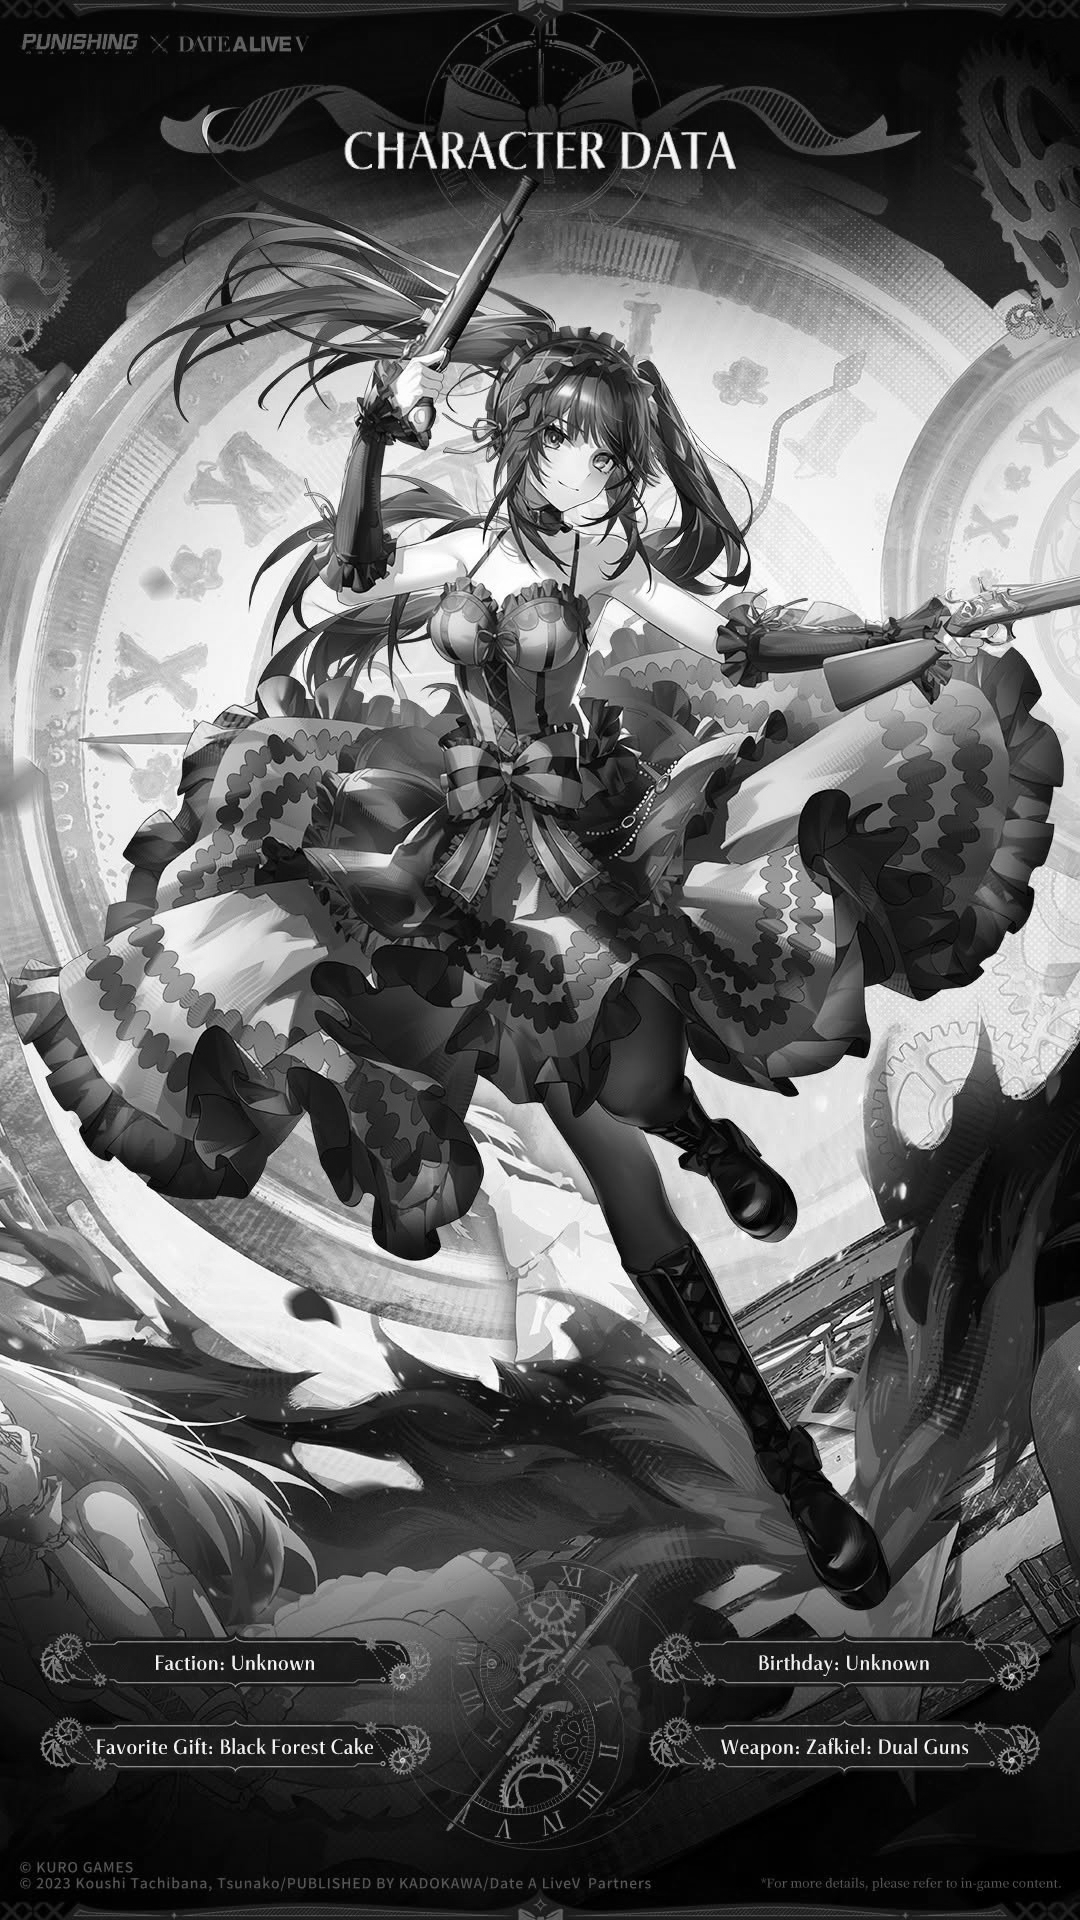
\includegraphics[width=0.85\textwidth]{grayscale.png}
\caption{Grayscale image produced by the first MAP operation.}
\label{fig:grayscale}
\end{figure}

\section{Finding Minimum and Maximum -- REDUCE}

After converting the image to grayscale, the minimum and maximum intensity values are required for the stretching operation.

The grayscale image is divided into 2D blocks. For each block, the implementation first calculates:

$$
min_{block} = \min(block)
$$

and

$$
max_{block} = \max(block)
$$

These partial results are then reduced to obtain the global minimum and maximum values:

$$
min = \min(min_{block_1},min_{block_2},\ldots)
$$

$$
max = \max(max_{block_1},max_{block_2},\ldots)
$$

This is the Reduce part of the implementation because multiple block-level values are combined to produce two global values.

For the input image used in this experiment, the measured values were:

$$
min = 0
$$

$$
max = 255
$$

\section{Grayscale Stretch -- MAP}

After obtaining the global minimum and maximum intensity, a second Map operation is performed.

For every grayscale pixel $g$, the new intensity is calculated as:

$$
g_0 =
\frac{g-\min}{\max-\min}
\times 255
$$

where $g$ is the original grayscale intensity, $\min$ is the global minimum intensity, and $\max$ is the global maximum intensity.

The result is clipped to the range $[0,255]$ and converted to the \texttt{uint8} data type.

The complete algorithm can therefore be represented as:

\begin{center}
\textbf{MAP}
$\rightarrow$
Grayscale Conversion
$\rightarrow$
\textbf{REDUCE}
$\rightarrow$
Global Min/Max
$\rightarrow$
\textbf{MAP}
$\rightarrow$
Grayscale Stretch
\end{center}

\begin{figure}[H]
\centering
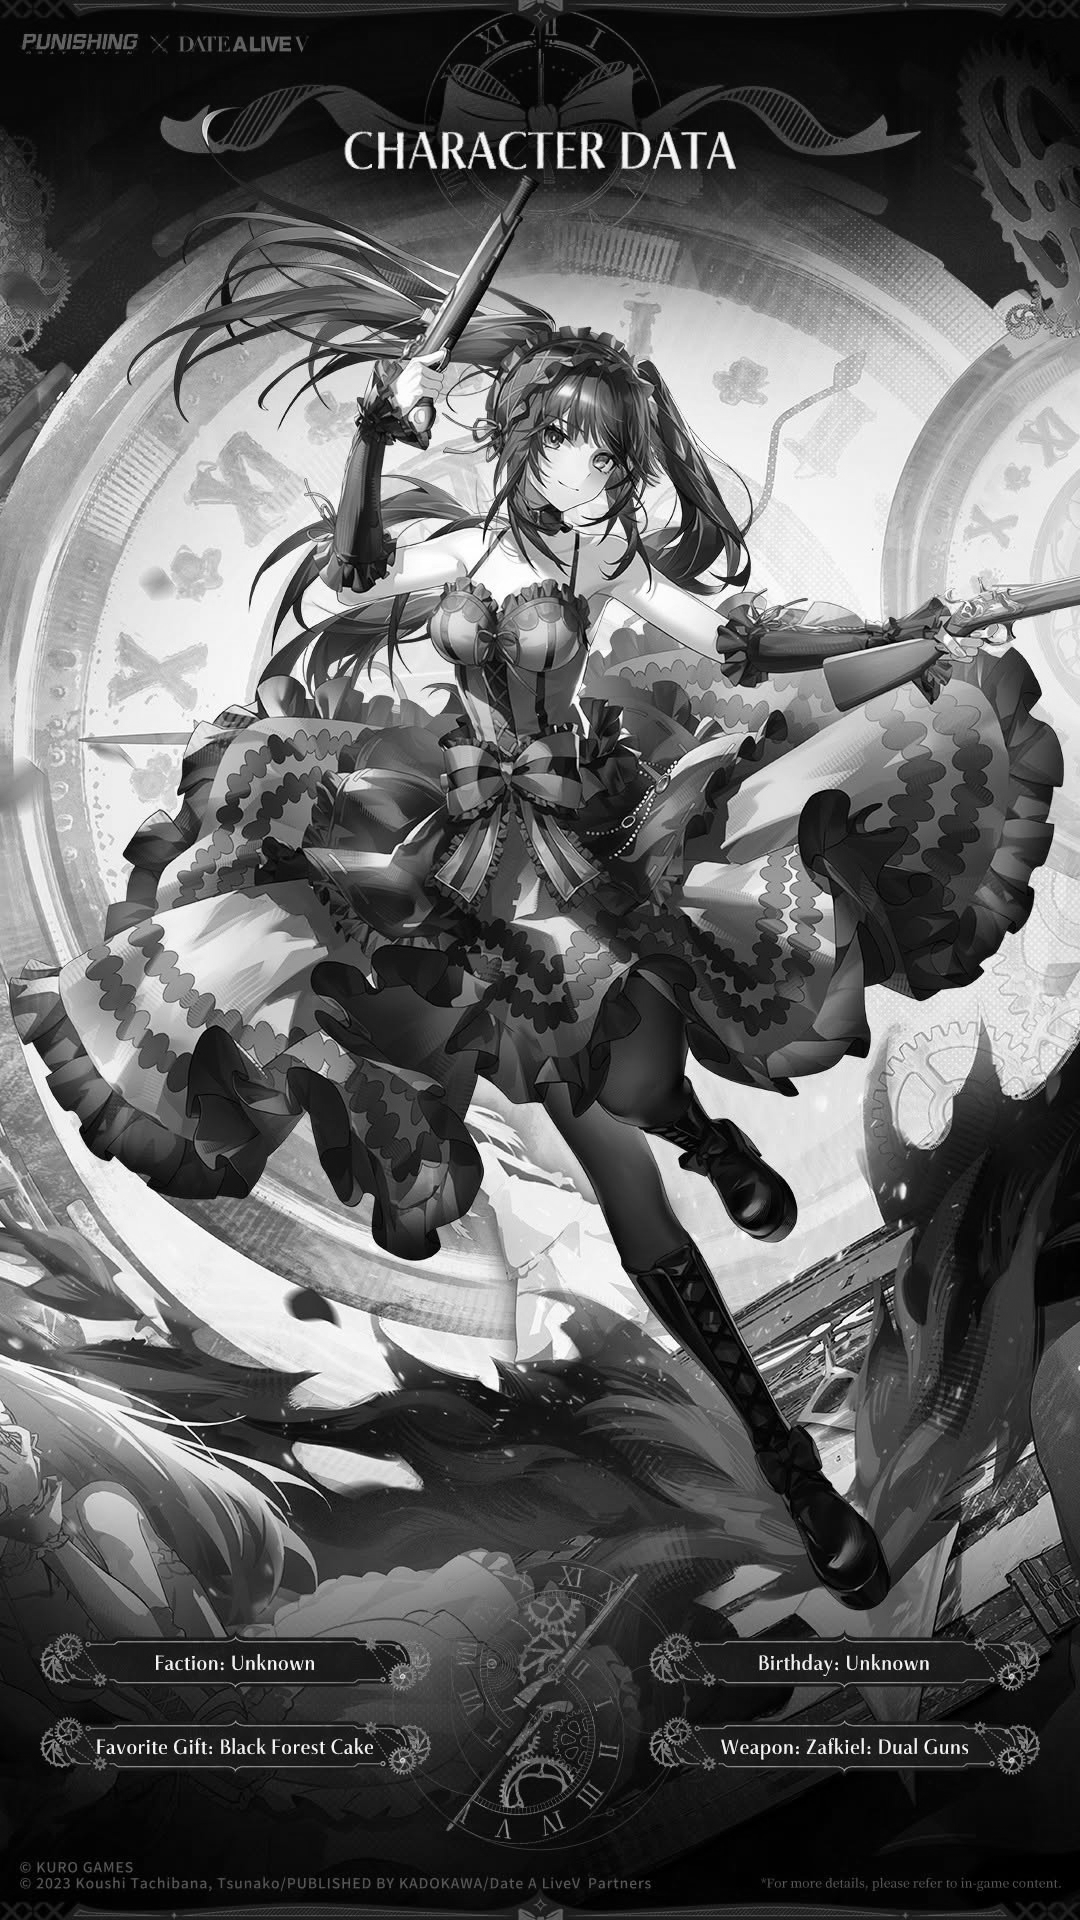
\includegraphics[width=0.85\textwidth]{grayscale_stretch.png}
\caption{Result of grayscale stretching.}
\label{fig:stretch}
\end{figure}

\section{Experiment with Different 2D Block Sizes}

The implementation was tested using five different 2D block sizes:

$$
4\times4,\quad
8\times8,\quad
16\times16,\quad
32\times32,\quad
64\times64
$$

For each block size, the complete grayscale stretch operation was executed and its execution time was measured.

\begin{table}[H]
\centering
\caption{Execution time for different 2D block sizes}
\label{tab:benchmark}
\begin{tabular}{ccccc}
\toprule
Block Size & Execution Time (s) & Min Intensity & Max Intensity \\
\midrule
$4\times4$   & 3.686888 & 0 & 255 \\
$8\times8$   & 1.200321 & 0 & 255 \\
$16\times16$ & 0.226212 & 0 & 255 \\
$32\times32$ & 0.077870 & 0 & 255 \\
$64\times64$ & 0.028527 & 0 & 255 \\
\bottomrule
\end{tabular}
\end{table}

A correctness check was also performed by comparing the output generated with each block size against the $16\times16$ result;f.

\begin{table}[H]
\centering
\caption{Correctness check for different block sizes}
\label{tab:correctness}
\begin{tabular}{cc}
\toprule
Block Size & Identical to $16\times16$ Result \\
\midrule
$4\times4$   & True \\
$8\times8$   & True \\
$16\times16$ & True \\
$32\times32$ & True \\
$64\times64$ & True \\
\bottomrule
\end{tabular}
\end{table}

\begin{figure}[H]
\centering
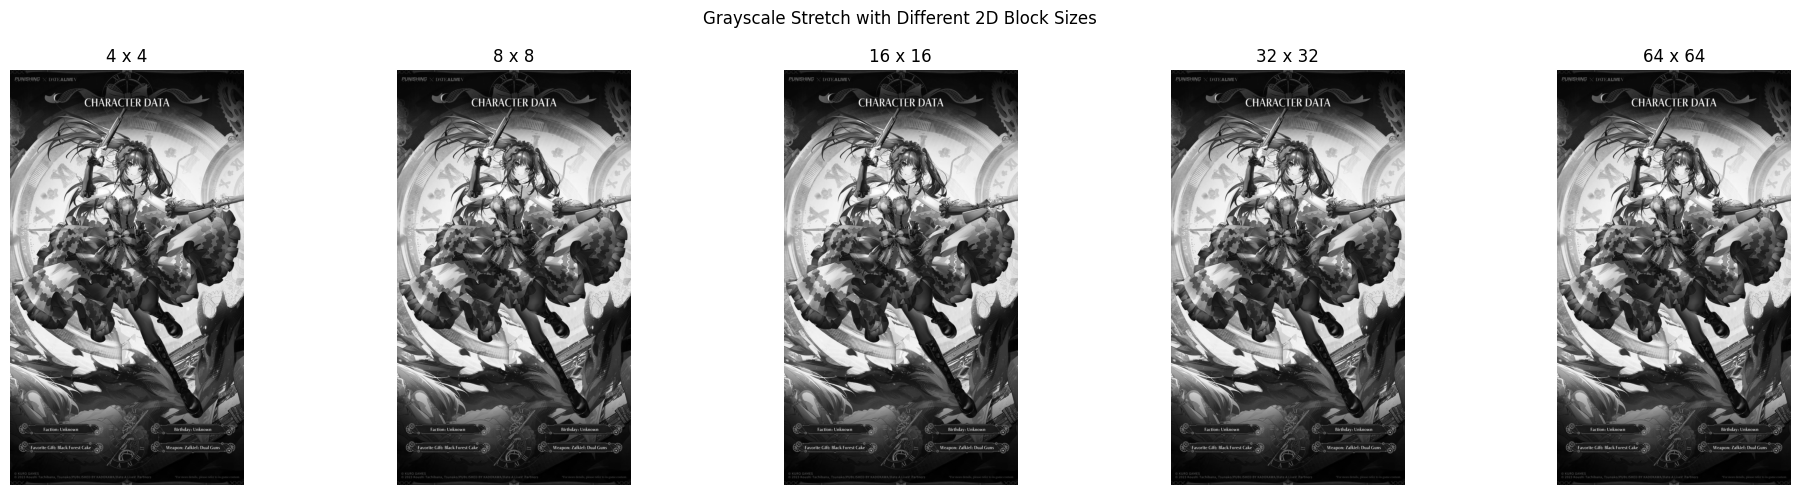
\includegraphics[width=0.95\textwidth]{grayscale_stretch_block_sizes.png}
\caption{Grayscale stretch results using different 2D block sizes.}
\label{fig:block_sizes}
\end{figure}

\section{Performance and Speedup}

The implementation measures the execution time for different block sizes. No separate optimized implementation was used for comparison, so a conventional speedup value is not calculated.

The measured execution times are reported in Table~\ref{tab:benchmark}. The block-size experiment is used to evaluate the execution performance of the implemented Map-Reduce approach.

\section{Conclusion}

In the labwork 7, grayscale stretching was implemented using a Map-Reduce style algorithm. The first Map operation converts the input image to grayscale. The Reduce operation calculates the global minimum and maximum grayscale intensities from the image blocks. Finally, a second Map operation applies the linear stretching formula to each pixel.

The implementation was tested with five different 2D block sizes. The correctness check showed that all tested block sizes produced the same grayscale stretch result as the $16\times16$ reference result.

\end{document}